\documentclass{article}
\usepackage{graphicx}
\usepackage{amsthm}
% \usepackage[yyyymmdd]{datetime}
\theoremstyle{definition}
\usepackage{mathtools}
\usepackage{natbib}
\usepackage{thmtools}
\usepackage[usenames, dvipsnames]{color}
\usepackage{algorithm}
\usepackage{algpseudocode}

\newtheorem{example}{Example}
\newtheorem{theorem}{Theorem}

\declaretheoremstyle[headfont=\bfseries]{solution}
\declaretheoremstyle[headfont=\normalfont]{normalhead}
\declaretheorem[style=normalhead, numbered=no]{question}
\declaretheorem[style=normalhead, numbered=no]{instance}
\declaretheorem[style=solution, numbered=no]{solution}

\title{The Traveller's Problem}
\author{Iva Babukova}

\begin{document}
\maketitle

In this work we present the Traveller's Problem (TP), a computational task whose extensions and variations are often encountered by travellers around the world. The task is concerned with creating a valid travel schedule, using airplanes as a means of transportation and in accordance with certain constraints specified by the traveller.

\section{Problem Formulation}
Each instance of TP consists of:

%% we may have either symmetric flight price (cost of fij = cost of fji) or asymmetric.

\begin{enumerate}
\item A set of airports $A = \{ A_{0},...,A_{n} \}$ \textcolor{red}{for $n > 0$}. Each airport $A_{i}$ $\in$ $A$ represents a location the traveller can begin their commute in, visit as a desired destination, or connect in on the way to their destination.
\textcolor{red}{Each airport $A_{i}$ has a \textit{connection time} $C_{A_{i}}$, that is the time that takes to commute to $A_{i}$.}
\item The trip starts and ends at the same airport $A_{0}$, which is referred to as the \textit{home point}.

\item The total travel time $T$, within which the traveller must have visited all destinations and returned to the home point.
 
\item A set of flights $F = \{ f_{0},...,f_{m} \}$. Each flight $f_{j}$ has:
\begin{itemize}
\item departure airport $A^{d}_{j}$,
\item arrival airport $A^{a}_{j}$,
\item date $t_{j}$,
\item duration \textcolor{red}{$\Delta_{j}$},
\item cost $c_{j}$,
\end{itemize} 
for some non-negative integer $j$ less than or equal to $n$.
The date $t_{j}$ is a positive \textcolor{red}{rational} number less than or equal to $T$ that shows at which day $f_{j}$ leaves its departure airport. The duration $\Delta{j}$ is a positive fraction that shows the amount of time that takes for flight $f_{j}$ to go from $A^{d}_{j}$ to $A^{a}_{j}$. The cost $c_{j}$ is a positive number that denotes the number of units of some currency $\epsilon$ that the traveller pays in order to be able to board flight $f_{j}$.

\item A set of \textit{destinations} \textcolor{red}{$D = \{ D_{1},...,D_{l} \}$, $D \subseteq A$, $l \leq n$}.
\end{enumerate}

A solution to any instance of TP is a sequence $s$ of $k$ valid flights, $\{f_{i_{1}}, f_{i_{2}},...,f_{i_{k}}\}\textcolor{red}{ \\ \subseteq F} $. We say that $s$ is valid if the flights in $s$ have the following properties:

\begin{enumerate}
\color{red}
\item $A^{d}_{i_{1}} = A^{a}_{i_{k}} = A_{0}$
\item $ A^{a}_{i_{j}} = A^{d}_{i_{j+1}},  \quad 0 < j < k  \quad j$
\item $ t_{i_{j}} + \Delta_{i_{j}} + C_{r} \leq t_{i_{j+1}}, \quad 0 < j \leq k, \quad \textrm{where } r = A^{a}_{i_{j+1}}$
\item $t_{i_{k}} + \Delta_{i_{k}} \leq T$
\item $ \forall D_{p} \in D, \textrm{ } \exists \textrm{ } f_{i_{j}} \in s \textrm{, such that } A^{a}_{i_{j}} = D_{p} $
\end{enumerate}

Note that a valid sequence of flights may contain \textcolor{red}{one} or more flights to and from airports that are not destinations. Such airports are called \textit{connections}.

\textcolor{red}{Also note that the current problem formulation accepts asymmetric flight costs, i.e. one might have two flights $f_{i}$ and $f_{j}$ such that $A^{d}_{i} = A^{a}_{j}$ and $A^{a}_{i} = A^{d}_{j}$. That does not imply that $c_{i} = c_{j}$. Moreover, the problem formulation does not restrict the flight cost to depend on the flight duration. Consequently, this implies that TP is \textit{asymmetric} and the flight cost does not satisfy the \textit{triangle inequality}.}

The \textit{optimization} version of TP (TPO) asks for an \textit{optimal} solution \textcolor{red}{$s$} which minimizes the total sum of the prices of the flights in $s$, denoted by $c(s)$.

The \textit{decision} version of TP (TPD) asks whether there exists a valid sequence of flights $s$, such that $c(s)$ is less than or equal to some \textcolor{red}{given} integer $B$. The solution of this problem is a `yes' or `no' answer.

There exist a variety of additional constraints and extensions that can be added to TP. Our problem formulation has only presented the hard constraints which every valid solution to a TP instance must satisfy. In real-world problems, travellers may have additional preferences (soft constraints) and requirements (hard constraints) with regards to their travel. These are discussed in the next two sections.

\subsection{Hard Constraints}
This section presents some additional constraints that might be imposed on a TP instance. If any of them is required, then a solution that does not satisfy the requirement is considered as invalid.

\begin{itemize}
\item \textcolor{red}{Travellers may wish to spend a certain amount of days at a given destination, specified by both upper and lower bounds. The days may additionally be constrained to be consecutive or not.}

\item Travellers may require to spend a given date at a given destination, for example due to an event occurring on that date in this destination.

\item \textcolor{red}{Travellers may require not to fly through a given airport more than once.}
%% TODO: delete this one maybe:
% \item Travellers may have a certain price threshold (budget) $B$, such that if the total travel cost exceeds that threshold the traveller will discard a solution as invalid.
\end{itemize}

\subsection{Soft Constraints}
It may be desirable to search for a solution that satisfies some of the following requirements:

\begin{itemize}
\item Travellers may wish to spend a certain amount $\delta_{i}$ of days in each destination $D_{i}$, where $\delta_{i}$ may be specified as a lower or an upper bound.

\item Travellers may wish to avoid taking connection flights. In such requirement, we wish to maximise the number of flights to and from destinations.

\item Travellers may want to spend as little time on flying as possible. In such case, we wish to find a solution that minimises the sum of the durations of all flights.
\end{itemize}

%% mention the problem with lexicographic optimisation and multi-objective opimisation
Note that we may have an instance for which all soft constraints can not be satisfied simultaneously. In such case, the traveller may be required to rank his requirements in an order of preference. The instance becomes a lexicographic optimisation problem, where \textcolor{red}{in addition to the highest priority constraint, we optimise also the second ranked constraint (provided that the previous one remains as optimal as possible) and so on for every constraint that needs to be satisfied.}
% \textcolor{red}{In such case, we might get solutions which are optimal with respect to the first constraint, but yield very poor results when trying to satisfy the lower ranked constraints.}
If all requirements are equally important for the traveller, we have to solve a multiobjective optimisation problem, where the objectives are all constraints required by the traveller. \textcolor{red}{Each of the objectives is given a weight of importance. The problem is then to optimize the objective function, composed by the constraints, each of them multiplied by its weight. Multiobjective and lexicographic optimisation problems are discussed later in this work.}

\textcolor{red}{Note that most of the aforementioned constraints can be viewed as either hard or soft, depending on the user requirements.}

It is therefore suggested that any attempt at an investigation of TP assumes as an additional non-functional requirement that any proposed model to solve TP is flexible and can be easily extended by adding, removing and modifying the aforementioned constraints.

\section{Worked Examples}
We present an example instance of TP and comment on some of its solutions.

\begin{example}
\label{example1}
A traveller wishes to visit 4 airports from a set of 7 airports available to travel to and from: 

Glasgow (G), Berlin (B), Milan (M), Amsterdam (A), Paris (P), Frankfurt (F), London (L).

Airport G is the home point, F and L are connections, and B, M, A and P are the destinations. The travel time of the traveller is 15 days. All available flights are listed on Table \ref{table:flights}. For simplicity, the duration of each flight is assumed to be 1 day. This means that if the traveller gets a flight at date $x$, they will reach the arrival airport at day $x+1$.

\begin{table}
\centering
\renewcommand{\arraystretch}{1.4}% Spread rows out...
\begin{tabular}{|l|c|c|c|c|c|}
\hline
\textbf{Flight No} & \textbf{Departs} & \textbf{Arrives} & \textbf{Date} & \textbf{Price} \\
\hline
GA1 & G & A & \date{1} & 74 \\
\hline
GF1 & G & F & \date{1} & 86 \\
\hline
FB2 & F & B & \date{2} & 156 \\
\hline
GL3 & G & L & \date{3} & 25 \\
\hline
MF3 & M & F & \date{3} & 78 \\
\hline
BP4 & B & P & \date{4} & 67 \\
\hline
AP4 & A & P & \date{4} & 58 \\
\hline
PM6 & P & M & \date{6} & 71 \\
\hline
FM8 & F & M & \date{8} & 234 \\
\hline
MF9 & M & F & \date{9} & 39 \\
\hline
FA10 & F & A & \date{10} & 220 \\
\hline
FB11 & F & B & \date{11} & 122 \\
\hline
FM12 & F & M & \date{12} & 250 \\
\hline
PL12 & P & L & \date{12} & 45 \\
\hline
BG13 & B & G & \date{13} & 335 \\
\hline
BL13 & B & L & \date{13} & 102 \\
\hline
AG13 & A & G & \date{13} & 90 \\
\hline
LG14 & L & G & \date{14} & 24 \\
\hline
\end{tabular}
\caption{List of flights with departure and arrival airports, flight date and price.}
\label{table:flights}
\end{table}
\end{example}

\begin{solution}
A valid solution of the TP instance in the example above is the sequence of flights $s$, where the each flight is represented by its flight number, specified in the first column of Table \ref{table:flights}:

$$ s = \{GA1, AP4, PM6, MF9, FB11, BG13\} $$

The total flights cost $c(s)$ is 699.

A valid solution with lower cost is the following sequence:

$$ s^{\prime} = \{GA1, AP4, PM6, MF9, FB11, BL13, LG14\} $$

\textcolor{red}{Here $c(s^{\prime})$ is 483 and hence $s$ is not optimal.}
\end{solution}

\begin{example}
\label{example2}
Given the same problem instance as in Example \ref{example1}, suppose that the traveller has booked a ticket for a concert in B on day 3. The traveller requires to attend the concert.
\end{example}

\begin{solution}
\textcolor{red}{In such case, neither $s$, nor $s^{\prime}$ from Example \ref{example1} are solutions}, because both of them assign the traveller to be at a different location (airport A) at day 3. The following sequence is a solution:

$$ s^{\prime\prime} = \{GF1, FB2, BP4, PM6, MF9, FA10, AG13\} $$

The total cost $c(s^{\prime\prime})$ is equal to 729, which is more expensive than $s$ and $s^{\prime}$.
\end{solution}

% \begin{example}
% \label{example3}
% \color{red}
% Given the same problem instance as in Example \ref{example1} and Example \ref{example2}, suppose that the traveller wishes to minimise the total cost of flights and the number of connection flights simultaneously.
% \end{example}

% \begin{solution}
% \color{red}
% We give a solution first using lexicographic optimisation and then multiobjective optimisation and comment on the advantages and disadvantages of the two methods.

% Lexicographic optimization


% Multiobjective optimization

% \end{solution}

\section{Use Cases}
\label{npcompleteproblems}

\textcolor{red}{This Section gives a list of known NP-complete problems \citep{thebible} referred to in this work when proving NP-hardness of TP (Section \ref{npcompleteproof}) and as use cases when reviewing the existing work (Section \ref{sec:existingwork}).}

\begin{enumerate}
\item \textbf{Travelling Salesman Problem (TSP)}

\begin{instance}
Set $A$ of $n$ cities, distance $d(A_{i}, A_{j})$ between each pair of cities $A_{i}$, $A_{j}$ $\in$ $A$ \textcolor{red}{that satisfies the triangle inequality}, positive integer $B$.
\end{instance}

\begin{question}
Is there a tour of $A$ having length $B$ or less, i.e., a permutation of cities $\gamma = A_{\pi(1)}, A_{\pi(2)},...,A_{\pi(n)}$ of $A$ such that
$$\bigg( \sum_{i=1}^{n-1} d(A_{\pi(i)}, A_{\pi(i+1)}) \bigg) + d(A_{\pi(n)}, A_{\pi(1)}) \leq B \quad \textrm{?}$$
\end{question}

\item \textbf{Time-Constrained TSP (TCTSP)}

\begin{instance}
Set $A$ of $n$ cities, distance d($A_{i}$, $A_{j}$) between each pair of cities $A_{i}$, $A_{j}$ $\in$ $A$, positive integer $B$, lower and upper bounds $l_{i}$ and $u_{i}$ respectively for each city $A_{i}$ that specify its time window.
\end{instance}

\begin{question}
It there a TSP tour such that for each city $A_{i}$ visited at time $t_{i}$, $l_{i} \leq t_{i} \leq u_{i}$ ?
\end{question}

\item \textbf{The Assignment Problem (AP)}

\begin{instance}
Set $A$ and set $B$ with equal size, cost $C(a,b)$ of matching $a \in A$ to $b \in B$.
\end{instance}

\begin{question}
Find a bijection $f: A \gets B$ such that $\sum_{a\in A} C(a,f(a))$ is minimised.
\end{question}
% \item \textbf{Vehicle-Routing Problem (VRP)}
% \item \textbf{Job-Shop Scheduling Problem (JSSP)}
% \item \textbf{Longest Path Problem}
\end{enumerate}


\section{Complexity of TP}

We state a theorem about the complexity of TP and prove it.

\begin{theorem}
The decision version of TP is NP-complete.
\end{theorem}

\begin{proof}
\label{npcompleteproof}
This proof first shows the membership of TPD in the NP class of problems. Second, we prove the NP-hardness of TP by constructing a polynomial-time reduction from a known NP-complete problem $\Pi$ to TPD, where $\Pi$ is chosen to be the traveling salesman problem (TSP), defined in Section \ref{npcompleteproblems}. Its NP-hardness follows by a reduction from the Hamiltonian Cycle problem. The proof is presented by \cite{thebible}.

Given an instance of TPD and $s$, which is a sequence of flights from $F$, we can write an algorithm $V$ that checks in polynomial time whether $s$ is a solution. To accept or reject validity, $V$ only needs to traverse $s$ and check that it satisfies all required properties. Therefore, TP is in NP.

Let $\pi$ be an instance of TSP, as defined in Section \ref{npcompleteproblems}. Let $\pi^{\prime}$ be an instance of TPD with the following properties:
\begin{itemize}
\item The set of airports in $\pi^{\prime}$ is identical to the set of cities in $\pi$ and it is similarly denoted as $A$ (a city in $\pi$ is called an airport in $\pi^{\prime}$).
\item Each airport in $A$ is also a destination.
\item The connection time $C_{A_{i}}$ for each airport $A_{i}$ is equal to 0.
\item $T$ is equal to $n+1$.
\item \textcolor{red}{Let $C$ be the Cartesian product of the airports in $A$ with itself, that is $C = A \times A$ = \{($A_{i}, A_{j}$) : $A_{i}$ $\in$ $A$, $A_{j}$ $\in$ $A$, $i \neq j$\}. Then $F$ is a set of flights, such that for every ($A_{i}, A_{j}$) $\in$ $C$, there exists a flight $f_{k}$ in $F$, such that $A^{d}_{k} = A_{i}$ and $A^{a}_{k} = A_{j}$ for every date $t \leq T$.}
\item For every $f_{k}$ $\in$ $F$, $c_{k}$ is equal to $d(A^{d}_{k}, A^{a}_{k})$ in $\pi$. \textcolor{red}{Therefore, the flights cost also satisfies the triangle inequality.} 
\item For every $f_{k}$ $\in$ $F$, $\Delta_{k}$ = 1.
\item $B$ is the upper bound on the allowed total cost.
\end{itemize}

%% TSP solution => also TP solution
\textcolor{red}{
Suppose that $\gamma$ = $A_{i_{1}}, A_{i_{2}},...,A_{i_{n}}$ is the most optimal solution of $\pi$, where $<i_{1},...,i_{n}>$ is a permutation of $<1,...,n>$ and the total travel distance $L_{\gamma} \leq B$. In $\pi^{\prime}$, $\gamma$ is equivalent to the order of visited airports by some sequence of flights $s$ = $f_{i_{1}}, f_{i_{2}},...f_{i_{n}}$, such that for every $f_{i_{k}} \in s, 1 \leq k \leq n$:}

\begin{itemize}
\color{red}
\item $ A^{d}_{i_{k}} = A_{i_{k}}, A_{i_{k}} \in \gamma $, and
\item $ A^{a}_{i_{k}} = A_{i_{k+1}}$, where subscripts are taken modulo $n$.
\end{itemize}

From the two conditions above it follows that $s$ satisfies property 1 and 2 of a valid solution. To satisfy property 3 and 4, it is sufficient to choose flights from $F$ such that for every $f_{k}$ $\in$ $s$, $t{k}$ = $k$. We know that such flights exist in $F$ by the construction of the set $F$. Property 5 is satisfied, since all airports in $A$ are destinations. Therefore, $s$ is a solution of $\pi^{\prime}$, from which it follows that a solution of $\pi$ is also a solution of $\pi^{\prime}$.

%% TP solution => also TSP solution
\textcolor{red}{Suppose that $s = \{f_{j_{1}},...,f_{j_{m}}\}$ is the most optimal solution of $\pi^{\prime}$, where flights in $s$ visit destinations in the sequence $\gamma^{\prime}$ = $\{A_{i_{1}}, A_{i_{2}},...,A_{i_{n}}\}$. We will prove that $\gamma^{\prime}$ is a solution of $\pi$. 
By construction of $\pi^{\prime}$, $\gamma^{\prime}$ contains all airports in A.
Suppose that an arbitrary airport $A_{s}$, for $i_{1} \leq s < i_{n}$, is included more than once in $\gamma^{\prime}$. Therefore, $A_{s}$ is listed at least twice in the tour: $\gamma^{\prime} = \{A_{i_{1}},...,A_{s-1},A_{s},...,A_{p},A_{s},A_{p+1}\}$ for $s < p < i_{n}$ and \\ $s=\{f_{i_{1}},...,f_{q},f_{q+1},...,f_{i_{m}}\}$. The tour is shown in Figure \ref{fig:routes}, where the green circles represent the airports, the red and black arrows are flights in $s$ and the purple flight $f_{r}$ in in $F$, but not in $s$. Since $s$ is the most optimal solution, $c_{q} + c_{q+1} < c_{r}$. However, by construction of $\pi^{\prime}$ the cost of the flights satisfies the triangle inequality and $c_{q} + c_{q+1}$ must be greater than $c_{r}$. This is a contradiction. Therefore, $A_{s}$ can not be added more than once to $\gamma^{\prime}$. Since $A_{s}$ was arbitrary chosen, the tour contains each airport in $A$ exactly once, which makes it a valid solution to $\pi$. Therefore, the most optimal solution of $\pi^{\prime}$ is a solution of $\pi$.}

\begin{figure}
\centering
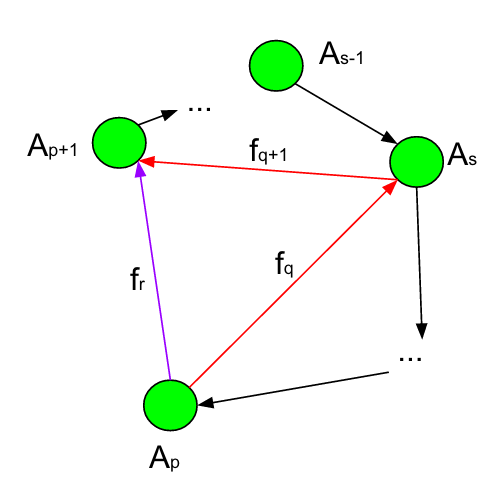
\includegraphics[width=6cm, height=6cm]{images/routes.png}
\label{fig:routes}
\caption{Tour $\gamma^{\prime}$}
\end{figure}

The transformation from a TSP instance to an instance of TP can be done in polynomial time. For each of the $n$($n$-1)/2 distances d($A_{i}$, $A_{j}$) that must be specified in $\pi$, it is sufficient to check that the same cost is assigned to the flights from $A_{i}$ to $A_{j}$ for all dates.

Therefore, TP is in NP and the decision version of TSP can be reduced to TPD in polynomial time, from which it follows that TPD is NP-complete.

\end{proof}

\section{Existing work}
\label{sec:existingwork}
We present some existing approaches to dealing with NP-hard problems, namely branch and bound (Section \ref{branchandbound}), constraint programming (Section \ref{cp}), approximation algorithms (Section \ref{approxalgos}) and integer programming (Section \ref{ip}). Each method is illustrated with the aid of a use case, listed in Section \ref{npcompleteproblems}.

\subsection{Branch and Bound Algorithms}
\label{branchandbound}
%% this is an enumerative method: The three most important enumerative methods are (i) implicit enumeration, (ii) dynamic programming, and (iii) branch and bound method
\textcolor{red}{
The origins of the branch and bound technique date back to the work by \citet{Dantzig54}, where an instance with 49 cities is solved and proved as optimal. The term ``branch and bound'' itself was introduced by \citet{Little63}.} 

\textcolor{red}{The branch and bound procedure repeatedly breaks up the set of feasible solutions into successively smaller subsets and calculates a \textit{bound} on the objective function value for each subset. The bounds are obtained by performing \textit{relaxation}, i.e. replacing the problem over a given subset with an easier (\textit{relaxed}) problem, such that the solution value of the latter bounds that of the former. Bounds are used to discard certain subsets from further consideration.}

% Let $P$ be an optimisation problem and let $v(P)$ be the value of the optimal solution to $P$. Any branch and bound procedure for $P$ of the form $min\{f(x) | x \in S\}$, where $S$ is the feasible set of $P$, has \citep{tspbible}:
% \begin{itemize}
% \item a \textit{relaxation} of $P$: a problem $R$ of the form $min\{f(x) | x \in T\}$, such that $S \subseteq T$ and for every $x, y \in S$, $f(x) < f(y)$ implies $g(x) < g(y)$.
% \item a \textit{branching rule}: a rule for breaking up the feasible set $S_{i}$ of the current subproblem $P_{i}$ into subsets $S_{i1},...,S_{iq}$ such that $\bigcup^{q}_{j=1} S_{ij} = S_{i}$.
% \item a \textit{lower bounding} procedure: a procedure for finding or approximating from below $v(R_{i})$ for the relaxation $R_{i}$ of each subproblem $P_{i}$.
% \item a \textit{subproblem selection rule}: a rule for choosing the next subproblem to be processed.
% \end{itemize}

% In addition, a branch and bound procedure may have an \textit{upper bounding} and \textit{testing} procedures. The former is a heuristic for finding feasible solutions to $P$, whereas the latter uses the logical implications of the problem constraints to discard subproblems as possible solutions or correct values of variables.
\textcolor{red}{
Branch and bound procedure can be represented as a rooted tree whose root node corresponds to the original problem and the leafs of the tree form the set of all candidate solutions. The successor nodes of each non-leaf node $i$ correspond to the subproblems, defined by the branching rule.}

\textcolor{red}{
Algorithm \ref{alg:branchandbound} presents a pseudo code of the branch and bound technique. An active problem set $s$ is set to contain the problem set initially (line 3). Then, we branch on each problem $P_{i}$ chosen from $s$. The branching rule generates a set of subproblems $s_{i}$ (line 10). Each subproblem $P_{ij}$ in $s_{i}$ is then checked whether it is ``worse'' than the best one found so far by calculating its bound (line 12, 13). Problems with ``worse'' bounds are being discarded (line 14), otherwise they are added to $s$ for further investigation (line 19). If the current bound is the ``best'' found so far, its value is remembered and used for comparison with next problems. On termination, the algorithm returns the most optimal solution of $P$ (line 23).}

%% pseudocode for branch and bound procedure:
\begin{algorithm}
\color{red}
\centering
\caption{Branch and Bound Procedure}
\label{alg:branchandbound}
\begin{algorithmic}[1]
\Procedure{BB }{Problem $P$}
\State \textbf{begin}
\State s $\gets$ \{$P$\} \Comment{\textit{put $P$ in the list of active problems set s}}
\State bestVal $\gets$ NULL
\State currentBest $\gets$ NULL
\State currVal $\gets$ NULL
\While{s \textbf{not} $\emptyset$}
\State $P_{i}$ $\gets$ \Call{choose}{s} \Comment{\textit{choose next subproblem}}
\State s $\gets$ s - $P_{i}$
\State $s_{i}$ = \Call{branch}{$P_{i}$} \Comment{\textit{branch on $P_{i}$, returns a list of subproblems}}
\For{$P_{ij}$ in $s_{i}$}
\State currVal $\gets$ \Call{bound}{$P_{ij}$} \Comment{\textit{calculate the bound of $P_{ij}$}}
\If{currVal \textbf{worse than} bestVal}
\State kill $P_{ij}$ \Comment{\textit{$P_{ij}$ can not lead to an optimal solution}}
\ElsIf{$P_{ij}$ is a complete solution}
\State bestVal $\gets$ currVal
\State currentBest $\gets$ $P_{ij}$
\Else
\State s $\gets$ s + $P_{ij}$
\EndIf
\EndFor
\EndWhile
\State \Return{currentBest}
\EndProcedure
\end{algorithmic}
\end{algorithm}

\textcolor{red}{
Algorithm \ref{alg:branchandbound} does not tell much about the ``choose'', ``branch'' and ``bound'' procedures. This is because there are many variations of their implementations. We discuss some of them in the following parts of this section.}

\subsubsection{Bounds based on the Assignment Problem}
This relaxation is based on expressing the integer programming version of an optimisation problem $P$ as an assignment problem (AP) after dropping one or more constraints from $P$.
The AP relaxation is successfully used for solving TSP \cite{Little63,Eastman58,Bellmore71,tspbible,Baker83} and for the Vehicle Routing Problem (VRP) \citep{Laporte86,vrpbible}. We explain the principles of this relaxation using TSP as a use case.

Let $P$ be an instance of TSP. The constraints of $P$ can be expressed with the following integer programming model \citep{tspbible,Dantzig54,Little63}:

Let $G(V,E)$ be a complete directed graph with vertex set $V = \{1,...,n\}$, where each vertex corresponds to a city in $P$ and set of edges $E = \{(i,j) | i,j \in V\}$ and non-negative cost $c(i,j)$ for each edge $(i,j)$ that is equal to the distance $d(i,j)$ in $P$. For all $i \in V$, $c(i,i) = \infty$ and for all edges $(i,j)$ that one wishes not to include in a tour, $c(i,j) = \infty$. Let $x(i,j)$ be either 1, if edge $(i,j)$ is in the solution, or 0 otherwise. Then, following \cite{Dantzig54}, $P$ can be formulated as the problem of minimising

\begin{equation}
\label{eq:one}
\sum_{i\in V}\sum_{j\in V} c(i,j)x(i,j)
\end{equation}

subject to

\begin{equation}
\label{eq:two}
\begin{split}
  \sum_{j \in V} x(i,j) = 1, \qquad i \in V,\\
  \sum_{i \in V} x(i,j) = 1, \qquad j \in V,
\end{split}
\end{equation}

\begin{equation}
\label{eq:subtourElimination}
\sum_{i\in S}\sum_{j\in S} x(i,j) \leq |S| - 1, \qquad \textrm{for all } S \subset V, S \neq \emptyset
\end{equation}

Equation (\ref{eq:two}) constrains that in a valid solution of $P$, each city has to be connected with exactly two cities. Note that formula (\ref{eq:two}) allows for solutions that include subtours, i.e. tours of length less than $n$. Equation (\ref{eq:subtourElimination}) is also known as \textit{subtour elimination} constraint and it serves the purpose to filter such invalid solutions.

In this formulation, one can remove constraint (\ref{eq:subtourElimination}) to obtain an instance of AP with the same cost function as $P$ \citep{Little63,Eastman58,Bellmore71}.

By dropping constraint (\ref{eq:subtourElimination}), the solution of $P_{AP}$ can be either a tour, or a collection of subtours. Hence, every tour of $P$ is a solution to AP, but not all solutions of AP are tours \citep{Bellmore71}. This allows for using the cost of the optimal solution of AP as a lower bound for the most optimal solution of $P$. In \cite{tspbible} it is showed with an experiment that both in theory and in practice the most optimal solution to AP is very likely to be a strong bound on $P$. The AP can be solved in at most $\mathcal{O}(n^{3})$ steps \citep{Kuhn55,Christofides75}. The ``bound'' procedure, that is called for every problem $P_{ij}$ in Algorithm \ref{alg:branchandbound}, computes AP$_{ij}$. It is shown in \cite{tspbible} that computing AP$_{ij}$ for each problem $P_{ij}$ in at most $\mathcal{O}(n^{2})$ steps by the Hungarian method \citep{Kuhn55}, provided that the algorithm is started from the optimal solution of the parent problem $P_{i}$.

%Performance

The AP relaxation is reported to perform differently, depending on the type of the problem \citep{tspbible,Bellmore71}. In particular, its performance highly depends on whether the problem has symmetric or asymmetric cost matrix. In the case with TSP, symmetric cost matrix refers to the property that the distance $d(i,j)$ from $i$ to $j$ is equal to $d(j,i)$. TSP with symmetric cost matrix is called Symmetric TSP (STSP) and Asymmetric TSP (ATSP) otherwise.

Experiments with ATSP instances have shown that the AP relaxation provides an excellent lower bound \citep{tspbible}. 

\subsubsection{Lagrangian relaxation}

\subsubsection{Choosing techniques}

\subsubsection{Branching rules}

% maybe remove this section
% \subsection{Dynamic Programming}
% \label{dynamicprogr}
% Use case: \cite{Christofides81}

\subsubsection{Performance of Branch and Bound Methods}
Until the late 1980s, the most effective exact approaches for the vehicle routing problem were mainly branch and bound algorithms \citep{vrpbible}.

\subsection{Approximation Algorithms}
\label{approxalgos}

\subsection{Constraint Programming}
\label{cp}
\subsubsection{Local Search}
\subsubsection{Heuristics}
\subsubsection{Use Case}
job-shop scheduling problem solution with CP

\subsection{Integer Programming}
\label{ip}

%%%%%%%%%%%%%%%%%%%%
%   BIBLIOGRAPHY   %
%%%%%%%%%%%%%%%%%%%%

\bibliographystyle{plainnat}
\bibliography{bib}

\end{document}







